\chapter{An Overview of Numerical Optimization}
\label{cha:overviewpart1}
In this chapter, we aim to provide readers an overview of numerical optimization. We begin with the theory of optimization (Section~\ref{sec:theory}), from the existence of optimizers, to the optimality conditions for both unconstrained and constrained problems with duality. This theoretical background of optimization provides a solid base for algorithm development. 
\par We then formally define the optimization of unconstrained and constrained problems in Section~\ref{sec:consopt} and describe the general regular solution for these problems based on the gradient calculation. 
\par Next, we briefly discuss the differentiable optimization in the neural network, which is a novel end-to-end network structure involving optimization problems in each layer with and without constraints. (Section~\ref{sec:differentiable}). Finally, we give a summary of the numerical optimization for solving unconstrained and constrained problems in Section~\ref{sec:2summary}.




\section{Theory of Optimization}
\label{sec:theory}
\subsection{Existence of Optimizers}
In optimization, a basic question is to determine the existence of a global optimizer. In this thesis, we focus on the optimizer in general minimization problems. Supposed we want to find the minimizer for a given function $f$. There are several sufficient conditions on $f$ to guarantee the existence, and the optimizer falls in the feasible set of solutions. For a feasible set, some related definitions are following: 
\begin{defn}~\citep{JS:06}
    A subset $\Omega \in \mathbb{R}^n$ is called
    \begin{itemize}
        \item \emph{bounded} if there is a constant $R > 0$ such that $\|x\| \leq R$ for all $x \in \Omega$
        \item \emph{closed} if the limit point of any convergent sequence in $\Omega$ always lies in $\Omega$
        \item \emph{compact} if any sequence $\left\{x_{k}\right\}$ in $\Omega$ contains a subsequence that converges to a point in $\Omega$
    \end{itemize}
\end{defn}
\par The following result gives a characterization of compact sets in $\mathbb{R}$. When we find the minimum or maximum solution for the problem, there exist a lower or upper bound but not necessarily an optimal solution. Therefore, we have some additional requirements. 
\par Firstly, we give the definition of compact sets in Lemma~\ref{lemma:bw}. ~\citep{OG:17} gives a brief proof.
\begin{lemma}[Bolzano-Weierstrass theorem]
    \label{lemma:bw}
    A subset $\Omega$ in $\mathbb{R}^n$ is \emph{compact} if and only if it is bounded and closed.
\end{lemma}
\par We also assume that the function $f$ is continuous and \emph{coercive}, where \emph{coercive} means "$+\infty$ at infinity". More precisely, $f(x) \rightarrow+\infty$ if $|x| \rightarrow+\infty$.~\citep{JS:06} Then the problem can be restricted to a bounded set and existence of a global minimum $x^{*}$ is guaranteed: a continuous function has a minimum on a compact set. This theorem is defined as follows and the proof is given in Appendix~\ref{appendix:trm23}.
\begin{thm}~\citep{JS:06}
    \label{thm:23}
    If $f$ is a continuous function defined on a compact set $\Omega$ in $\mathbb{R}$, then $f$ has a global minimizer $x^{*}$ on $\Omega$ i.e. there exists $x^{*} \in \Omega$ such that $f\left(x^{*}\right) \leq f(x)$ for all $x \in \Omega$.
\end{thm}
More general, based on the definition of coercive function $f$, we can give following theorem. Proof is given in Appendix~\ref{appendix:trm24}.
\begin{thm}~\citep{JS:06}
    \label{thm:24}
    If $f: \mathbb{R}^{n} \rightarrow \mathbb{R}$ is a continuous coercive function, then $f$ has at least one global minimizer.
\end{thm}
Theorem~\ref{thm:24} requires the continuity of $f$ which is slightly restrictive for applications. However, we can replace it by the lower semi-continuity of $f$ which is a rather weaker condition. 
\begin{defn}~\citep{JS:06}
    Let $f: \mathbb{R}^{n} \rightarrow \mathbb{R} \cup\{\pm \infty\}$. Then $f$ is called \emph{lower semi-continuous} at a point $x_0 \in \mathbb{R}^n$ if for any sequence $f\left(x_{k}\right)$ converging to $x_0$ here holds $f\left(x_{0}\right) \leq \lim _{k \rightarrow \infty} f\left(x_{k}\right)$. $f$ is called \emph{lower semi-continuous} if $f$ is lower semi-continuous at every point.
\end{defn}
Recall our assumptions on function $f$, it is a continuous function, which is always lower semi-continuous. Notably, lower semi-continuous functions are not necessarily continuous. For instance, a binary function equals to 0 when $x \leq 0$ and equals to 1 when $x > 0$ is not continuous at $x_0 = 0$. However, since it is greater than 0 for all $x$ and $f(0) = 0$, we have $f(0)=0 \leq \liminf _{x \rightarrow 0} f(x)$ and it is lower semi-continuous at $x_0 = 0$.
\par The theorem of the existence of the optimizer of lower semi-continuous function is given as follows and the proof is given in Appendix~\ref{appendix:thm25}
\begin{thm}~\citep{JS:06}
    \label{thm:25}
    Let $f: \mathbb{R}^{n} \rightarrow \mathbb{R}$ be a lower semi-continuous function. If $f$ has a nonempty, compact sublevel set $D:=\left\{x \in \mathbb{R}^{n}: f(x) \leq \alpha\right\}$, then $f$ achieves a global minimizer on $\mathbb{R}$.
\end{thm}
Also, we introduce the definition of convex function and convex set which are important in regular optimization problems.
\begin{defn}~\citep{JS:06}
    A function $f$ is convex when 
    $$
        f(\alpha x+(1-\alpha) y) \leq \alpha f(x)+(1-\alpha) f(y) \quad \textrm{for all } x, y, \textrm{ and } \alpha \in ]0,1[
    $$
    A set $C \subset \mathbb{R}^n$ is convex when 
    $$
    \alpha x+(1-\alpha) y \in C \quad \textrm { for all } x, y \textrm { in } C, \textrm{ and } \alpha \in ] 0,1[
    $$
\end{defn}
The objective function of the optimization problem we discussed in this part is convex and regular, which means its gradient can be computed and the solution exists. However, although the existence of the optimizer is sufficient, for unconstrained and constrained problems, the optimality conditions are different. In the next two sections, we will give necessary and sufficient conditions for both these cases. 

\subsection{Optimality Conditions for Unconstrained Problems}
Firstly, we consider the unconstrained minimization problem
\begin{equation}
    \min _{\mathbf{x} \in \mathbb{R}^{n}} f(x),
\end{equation}
where $f$ is the objective function on $\mathbb{R}^n$. 
\par In order to determine the minimizer, it is important to understand what can happen at a minimizer, and at what conditions a point must be a minimizer. Now we have to recognize the optimal point. There are two necessary conditions and one sufficient condition given below~\citep{JS:06}. The proof is given in Appendix~\ref{appendix:thm28}.
\begin{thm}{Necessary and Sufficient Conditions.}
    \label{thm28}
    Let $f:\Omega \rightarrow \mathbb{R}$ be a funcion defined on a set $\Omega \subset \mathbb{R}^n$ and let $x^*$ be an interior point of $\Omega$ that is a local minimizer of $f$. \\
    Necessary conditions:
    \begin{itemize}
        \item (NC1) If $f$ is differentiable at $x^*$, then $x^*$ is a critical point of $f$, i.e. $\nabla f\left(x^{*}\right)=0$.
        \item (NC2) If $f$ is twice continuous differentiable on $\Omega$, then the Hessian $\nabla^2 f\left(x^{*}\right)$ is positive semidefinite.
    \end{itemize}
    Sufficient condition (SC1): if $x^*$ is such that $\nabla f\left(x^{*}\right)=0$ and $\nabla^2 f\left(x^{*}\right)$ is positive definite, then $x^*$ is a local minimum. (i.e. $f(x) \geq f(x^*)$ for $x$ close to $x^*$)
\end{thm}
\par Any point satisfying (NC1) as the minimizer of $f$ is called a \emph{critical} or \emph{stationary} point of $f$. If the objective function $f$ is convex, (NC1) is also the sufficient condition for the global minimum of the solution. 
\par Below is an example of unconstrained minimization problem. Supposed we have to determine the minimum of function
$$
f(x, y)=x^{4}-4 x y+y^{4}
$$
\par From the definition of function $f$, it is clear that $f$ is continuous, then we can expand $f$ by writing
$$
f(x, y)=\left(x^{4}+y^{4}\right)\left(1-\frac{4 x y}{x^{4}+y^{4}}\right)
$$
\par we can see $f$ is coercive. Also, we show the contour graph of function $f$ in Figure~\ref{fig:unconseg}. Therefore $f$ has global minimizers which are critical points. According to (NC1), we can find the global minimizer through solving the derivative of $f$ equaling to zero:
$$
0=\nabla f(x, y)=\left(\begin{array}{c}4 x^{3}-4 y \\ -4 x+4 y^{3}\end{array}\right)
$$
\par Thus, $y = x^3$ and $x = y^3$. Consequently $y = y^9$, i.e.
$$
0=y-y^{9}=y\left(1-y^{8}\right)=y\left(1-y^{4}\right)\left(1+y^{4}\right)=y(1-y)(1+y)\left(1+y^{2}\right)\left(1+y^{4}\right)
$$
\par This implies $y = 0, 1, -1$. Thus $f$ has three critical points $(0,0), (1,1), (-1,-1)$. Then we can evaluate $f$ as these points since they may be local minimizer:
$$
f(0,0)=0, \quad f(1,1)=-2, \quad f(-1,-1)=-2
$$
\par It achieves the same global minimum value on $(1, 1)$ and $(-1, -1)$. Therefore, they are both global minimizers of $f$. Figure~\ref{fig:example12_solution} shows the function $f(x,y)$ at these two optimal points. 
\begin{figure}[t]
\label{fig:unconseg}
\centering
    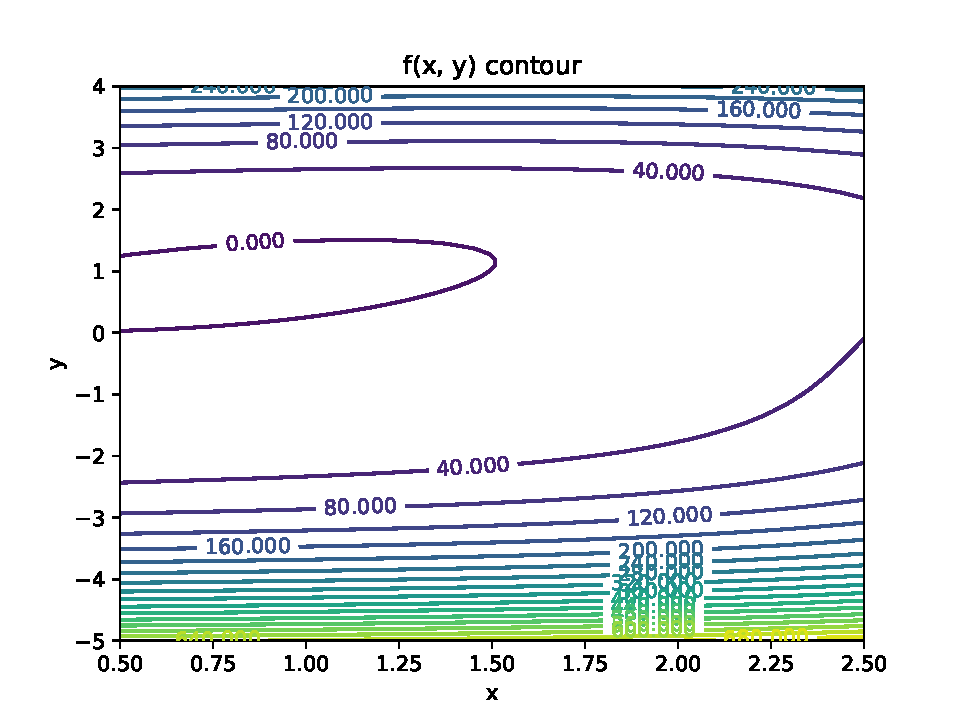
\includegraphics[page=1,width=.7\columnwidth]{figs/contour_21.pdf}
\caption{Contour Graph of $f(x, y)=x^{4}-4 x y+y^{4}$}
\end{figure}
\begin{figure}[t]
    \label{fig:example12_solution}
    \centering
    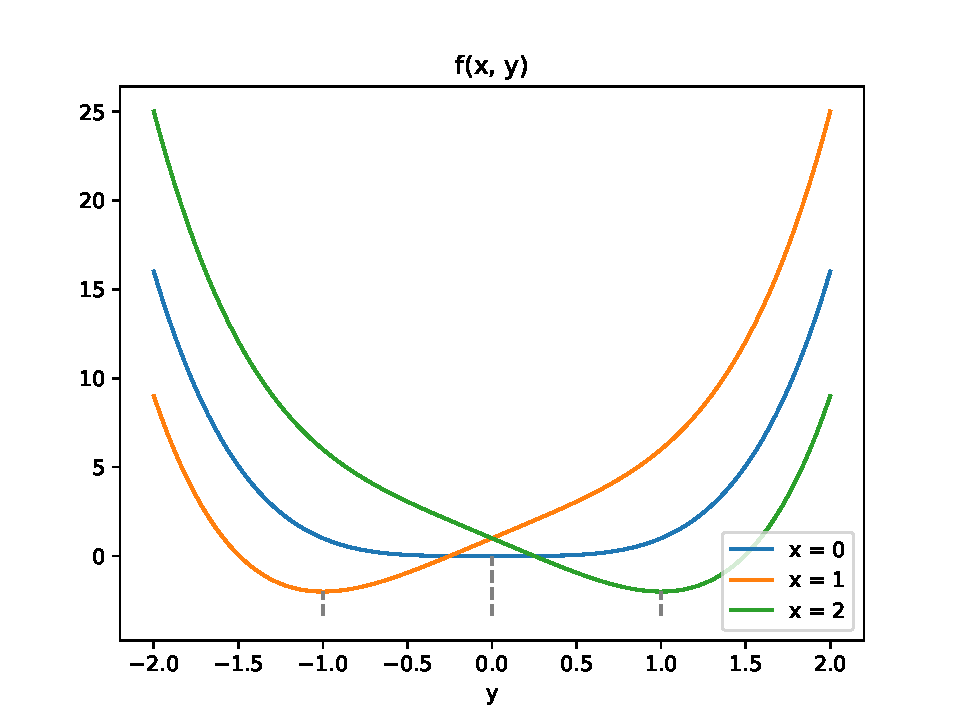
\includegraphics[page=1,width=.7\columnwidth]{figs/solution_21.pdf} 
  \caption{Function $f(x,y)$ at $x = 0$, $x=-1$ and $x=1$ }
 \end{figure}

\par From this example, we verify that we can find the global minimizer through (NC1). However, not all continuous functions with critical points have a global maximizer or minimizer. If the function goes to infinity along its axes or a line, it does not have any maximizer or minimizer although it has a critical point, such as the cubic function. The condition of the minimizer as the critical point is that the function $f$ should be a convex function with continuous first partial derivatives.
\par Let us move to the sufficient condition (SC1). The result obtained under this theorem is best possible for general functions. Specifically, for a convex function $f$ that is defined on a convex set $\Omega \subset \mathbb{R}^n$, any local minimizer of $f$ is also a global minimizer. Moreover, if a function $f$ is strictly convex, it has at most one global minimizer. 

\subsection{Optimality Conditions for Constrained Problems}
\label{sec:opt-con-constrained}
A general formulation for constrained optimization problems is as follows: 
\begin{equation}
\label{equ:2.2}
\begin{array}{l}\textrm { minimize } f(x) \\ \textrm { subject to }\left\{\begin{array}{ll}c_{i}(x)=0 & \textrm { for } i=1, \cdots, m_{e}, \\ c_{i}(x) \leq 0 & \textrm { for } i=m_{e}+1, \cdots, m\end{array}\right.\end{array}
\end{equation}
where $f$ and $c_i$ are smooth real-valued functions on $\mathbb{R}^n$, and $m_e$ and $m$ are nonnegative integers with $m_e < m$. We set 
$$
\mathscr{E}:=\left\{1, \cdots, m_{e}\right\} \quad \textrm { and } \quad \mathscr{I}:=\left\{m_{e}+1, \cdots, m\right\}
$$
as index sets of equality constraints and inequality constraints, respectively. 
\par Here, $f$ is so-called the objective function, and $c_i, i \in \mathscr{E} \textrm{ and } \mathscr{I}$ are equality constraints and inequality constraints respectively. 
\par To solve the optimization problem (\ref{equ:2.2}), we define the feasible set of it to be
$$
\mathscr{F}:=\left\{x \in \mathbb{R}^{n}: c_{i}(x)=0 \textrm { for } i \in \mathscr{E} \textrm { and } c_{i}(x) \leq 0 \textrm { for } i \in \mathscr{I}\right\}
$$
\par Any point $x \in \mathscr{F}$ is called a feasible point of (\ref{equ:2.2}) and we call (\ref{equ:2.2}) infeasible if $\mathscr{F} = 0$. Also, in this feasible set, a feasible point $x^* \in \mathscr{F}$ is called a local minimizer of (\ref{equ:2.2}) if it is the minimum solution in a neighborhood (strict local minimizer if it is the only one minimum solution). The definition of the global minimizer and strict global minimizer is similar, whose neighborhood is the whole feasible set. 
\par Let us move to the constraints in this problem. For equality constraints, they are strictly equivalent. However, for inequality constraints, there are some exceptions. Let $x^*$ be a local minimizer of (\ref{equ:2.2}). If there is an index $i \in \mathscr{I}$ such that $c_i(x^*) < 0$, then, $x^*$ is still the local minimizer of the problem obtained by deleting $i$-th constraint. In this situation, we say that the $i$-th constraint is inactive at $x^*$ since it does not have any effect on the solution. A general definition of active and inactive inequality constraints is as follows:
\begin{defn}~\citep{JS:06}
    At a feasible point $x \in \mathscr{F}$, the index $i \in \mathscr{I}$ is said to be \emph{active} if $\mathscr(x) = 0$ and \emph{inactive} if $c_i(x) < 0$.  
\end{defn}
\par In the next chapter, we will give different processes for different cases of active or inactive inequality constraints in the deep declarative nodes. In this chapter, we only focus on the necessary and sufficient conditions for a feasible point $x$ to be a local minimizer of (\ref{equ:2.2}). These conditions will be derived by considering the change of $f$ on the feasible set along with certain directions. We give the lemma for the condition of local minimizer $x^* \in \mathscr{F}$ as follows, which can be proved through Taylor’s formula in Appendix~\ref{appendix:lemma210}.
\begin{lemma}~\citep{JS:06}
    \label{lemma:210}
    If $x^* \in \mathscr{F}$ is a local minimizer of (\ref{equ:2.2}), then
    $$
    d^{T} \nabla f\left(x^{*}\right) \geq 0 \quad \textrm { for all } d \in T_{x^{*}} \mathscr{F}
    $$
    where $T_{x^{*}} \mathscr{F}$ is the set of all vectors tangent to $\mathscr{F}$. 
\end{lemma}
\par However, we may not be able to extract useful results from this lemma, since $T_{x^{*}} \mathscr{F}$ depends only on the geometry of $\mathscr{F}$ but not on the constraints functions $c_i$. Not all local minimum falls on the boundary of the constraint function, which is a part of $T_{x^{*}} \mathscr{F}$. Therefore, it is necessary to introduce linearized feasible directions to give a characterization of $T_{x^{*}} \mathscr{F}$ in terms of $c_i$. 
\begin{defn}~\citep{JS:06}
    \label{defn:lfd}
    Given $x \in \mathscr{F}$, we define
    $$
    \operatorname{LFD}(x):=\left\{d \in \mathbb{R}^{n}: d^{T} \nabla c_{i}(x)=0 \text { for } i \in \mathscr{E} ; d^{T} \nabla c_{i}(x) \leq 0 \textrm { for } i \in \mathscr{I} \cap \mathscr{A}(x)\right\}
    $$
    and call it the set of linearized feasible directions of $\mathscr{F}$ at $x$. 
\end{defn}
\par Heuristically, for $i \in \mathscr{E}$ we should travel along directions $d$ with $d^{T} \nabla c_{i}(x)=0$ in order to stay on the curve $c_i(x)=0$; for $i \in \mathscr{I}$ we should travel along directions with $d^{T} \nabla c_{i}(x) \leq 0$ in order to stay in the region $c_i(x) \leq 0$. 
Let us see an example of the linearized feasible directions and the tangent. Supposed we are considering a set $\mathscr{F}$ with variables $(x,y) \in \mathbb{R}^2$ and three inequality constraints functions: 
$$
\begin{aligned}
    c_1(x,y) &= x-1 \leq 0 \\
    c_2(x,y) &= -y \leq 0\\
    c_3(x,y) &= y^2 - x \leq 0
\end{aligned}
$$
\begin{figure}[t]
    \label{fig:example22_set}
    \centering
    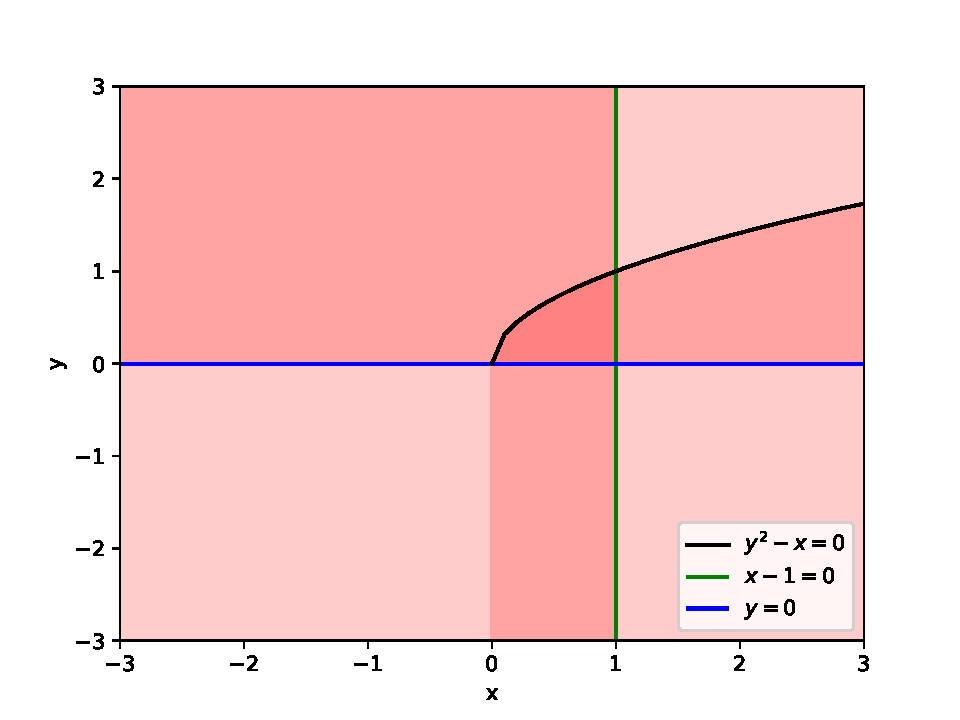
\includegraphics[page=1,width=.7\textwidth]{figs/solution_22.pdf} 
  \caption{Feasible set of constraints $c_1$, $c_2$ and $c_3$}
\end{figure}

\par We can illustrate the feasible set of constriants $c_1$, $c_2$ and $c_3$ in Fig~\ref{fig:example22_set}. The active set of $0=(0,0)$ is $\{2, 3\}$, since $c_1(0) = -1 < 0$, which is inactive. And we can get the derivative of $c_2$ and $c_3$ at 0: 
$$
\nabla c_{2}(0)=(0,-1)^{T} \quad \textrm { and } \quad \nabla c_{3}(0)=(-1,0)^{T}
$$
\par Then we have the linearized feasible directions on $x=0$: 
$$
\begin{aligned} \operatorname{LFD}(0) &=\left\{d \in \mathbb{R}^{2}: d^{T} \nabla c_{2}(0) \leq 0 \text { and } d^{T} \nabla c_{3}(0) \leq 0\right\} \\ &=\left\{d \in \mathbb{R}^{2}: d \geq 0\right\} \end{aligned}
$$
which equals the set of all vectors tangent to the feasible set $T_{0} \mathscr{F}$. 
\par Unlike the unconstrained optimization problem, the first order necessary condition of the existence of the optimizer is different since we should consider its linearized feasible directions and constraints feasibility. This is so-called the Karush-Kuhn-Tucker theorem: 
\begin{thm}[Karush-Kuhn-Tucker Theorem]~\citep{JS:06}
    \label{thm:kkt}
    Let $x^* \in \mathscr{F}$ be a local minimizer of problem (\ref{equ:2.2}). If
    $$
    T_{x^*} \mathscr{F} = \operatorname{LFD}(x^*),
    $$
    then there exists $\lambda^{*}=\left(\lambda_{1}^{*}, \cdots, \lambda_{m}^{*}\right)^{T} \in \mathbb{R}^{m}$ such that 
    $$
    \nabla f\left(x^{*}\right)+\sum_{i \in \mathscr{E} \cup \mathscr{I}} \lambda_{i}^{*} \nabla c_{i}\left(x^{*}\right)=0, \quad(\textrm {Lagrangian stationary})
    $$
    $$
    \left.\begin{array}{ll}c_{i}\left(x^{*}\right)=0 & \text { for all } i \in \mathscr{E}, \\ c_{i}\left(x^{*}\right) \leq 0 & \text { for all } i \in \mathscr{I},\end{array}\right\} \quad(\textrm {primal feasibility})
    $$
    $$
    \lambda_{i}^{*} \geq 0 \quad \textrm {for all} i \in \mathscr{I}, \quad (\textrm {dual feasibility})
    $$
    $$
    \lambda_i^*c_i(x^*) = 0 \quad \textrm {for all} i \in \mathscr{E} \cup \mathscr{I}. \quad (\textrm {complementary slackness})
    $$
    This set of equations are Karush-Kuhn-Tucker (KKT) conditions and a point $x^*$ is called a KKT point if there exists $\lambda^*$ such that $(x^*, \lambda ^*)$ satisfies the KKT conditions.
\end{thm}
\par For constrained optimization problem, the classic solution is using Lagrange multipliers \citep{BD:14}. Figure~\ref{fig:lagrange-example} shows an example of constrained problem, where $f(x, y) = d_i, i = 1, 2, 3$ are the contours of different solution of the objective function and $c(x,y) = 0$ is the equality constraint of the problem. 
\begin{figure}[t]
    \label{fig:lagrange-example}
    \centering
    \tikzset{every picture/.style={line width=0.75pt}} %set default line width to 0.75pt        
    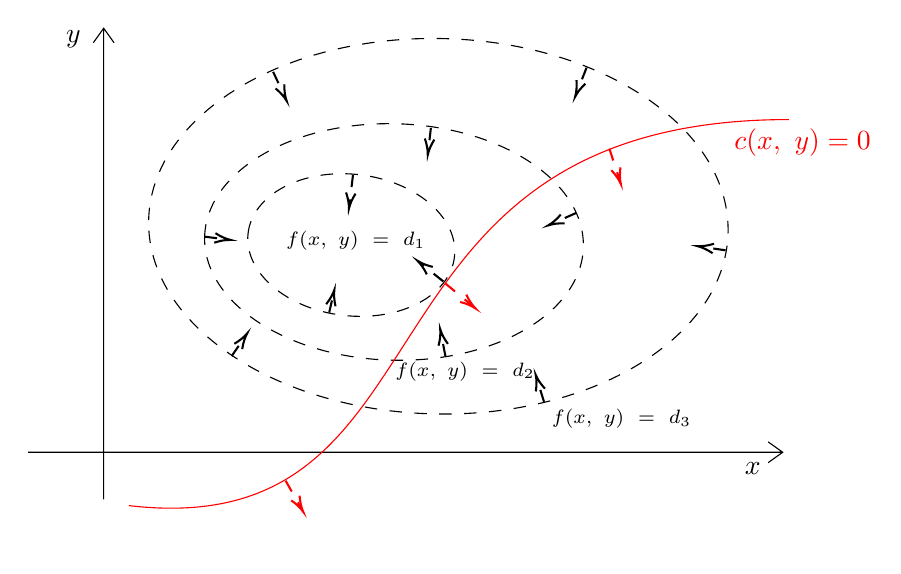
\begin{tikzpicture}[x=0.75pt,y=0.75pt,yscale=-1,xscale=1]
        %uncomment if require: \path (0,300); %set diagram left start at 0, and has height of 300

        %Shape: Axis 2D [id:dp5517214573358842] 
        \draw  (149,249.3) -- (512.5,249.3)(185.35,45) -- (185.35,272) (505.5,244.3) -- (512.5,249.3) -- (505.5,254.3) (180.35,52) -- (185.35,45) -- (190.35,52)  ;
        %Shape: Ellipse [id:dp22516389660099345] 
        \draw  [dash pattern={on 4.5pt off 4.5pt}] (254.92,143.8) .. controls (257.05,125.08) and (281.04,112.44) .. (308.49,115.56) .. controls (335.95,118.69) and (356.48,136.39) .. (354.36,155.11) .. controls (352.23,173.83) and (328.24,186.47) .. (300.78,183.34) .. controls (273.33,180.22) and (252.79,162.52) .. (254.92,143.8) -- cycle ;
        %Shape: Ellipse [id:dp49554237272610546] 
        \draw  [dash pattern={on 4.5pt off 4.5pt}] (233.99,145.42) .. controls (234.87,113.97) and (276.43,89.62) .. (326.82,91.04) .. controls (377.21,92.45) and (417.34,119.1) .. (416.46,150.55) .. controls (415.57,182) and (374.01,206.34) .. (323.62,204.93) .. controls (273.23,203.51) and (233.1,176.87) .. (233.99,145.42) -- cycle ;
        %Shape: Ellipse [id:dp7806828933868084] 
        \draw  [dash pattern={on 4.5pt off 4.5pt}] (207.02,137.45) .. controls (208.08,87.51) and (271.42,48.35) .. (348.51,49.98) .. controls (425.6,51.61) and (487.24,93.41) .. (486.18,143.35) .. controls (485.13,193.28) and (421.78,232.45) .. (344.69,230.82) .. controls (267.6,229.19) and (205.97,187.39) .. (207.02,137.45) -- cycle ;
        %Curve Lines [id:da36285843872545764] 
        \draw [color={rgb, 255:red, 255; green, 0; blue, 0 }  ,draw opacity=1 ]   (197.5,275) .. controls (360.5,294) and (296.5,89) .. (515.5,89) ;
        %Straight Lines [id:da4302907773489495] 
        \draw [line width=0.75]  [dash pattern={on 4.5pt off 4.5pt}]  (267,66) -- (272.66,78.19) ;
        \draw [shift={(273.5,80)}, rotate = 245.1] [color={rgb, 255:red, 0; green, 0; blue, 0 }  ][line width=0.75]    (7.65,-2.3) .. controls (4.86,-0.97) and (2.31,-0.21) .. (0,0) .. controls (2.31,0.21) and (4.86,0.98) .. (7.65,2.3)   ;
        %Straight Lines [id:da6345979393684194] 
        \draw [line width=0.75]  [dash pattern={on 4.5pt off 4.5pt}]  (418,64) -- (413.23,76.14) ;
        \draw [shift={(412.5,78)}, rotate = 291.45] [color={rgb, 255:red, 0; green, 0; blue, 0 }  ][line width=0.75]    (7.65,-2.3) .. controls (4.86,-0.97) and (2.31,-0.21) .. (0,0) .. controls (2.31,0.21) and (4.86,0.98) .. (7.65,2.3)   ;
        %Straight Lines [id:da7677780782766945] 
        \draw [line width=0.75]  [dash pattern={on 4.5pt off 4.5pt}]  (485,152) -- (473.48,150.29) ;
        \draw [shift={(471.5,150)}, rotate = 368.43] [color={rgb, 255:red, 0; green, 0; blue, 0 }  ][line width=0.75]    (7.65,-2.3) .. controls (4.86,-0.97) and (2.31,-0.21) .. (0,0) .. controls (2.31,0.21) and (4.86,0.98) .. (7.65,2.3)   ;
        %Straight Lines [id:da8512837599521172] 
        \draw [line width=0.75]  [dash pattern={on 4.5pt off 4.5pt}]  (397.5,225) -- (394.09,213.91) ;
        \draw [shift={(393.5,212)}, rotate = 432.9] [color={rgb, 255:red, 0; green, 0; blue, 0 }  ][line width=0.75]    (7.65,-2.3) .. controls (4.86,-0.97) and (2.31,-0.21) .. (0,0) .. controls (2.31,0.21) and (4.86,0.98) .. (7.65,2.3)   ;
        %Straight Lines [id:da3071908779325687] 
        \draw [line width=0.75]  [dash pattern={on 4.5pt off 4.5pt}]  (247,203) -- (253.37,193.65) ;
        \draw [shift={(254.5,192)}, rotate = 484.29] [color={rgb, 255:red, 0; green, 0; blue, 0 }  ][line width=0.75]    (7.65,-2.3) .. controls (4.86,-0.97) and (2.31,-0.21) .. (0,0) .. controls (2.31,0.21) and (4.86,0.98) .. (7.65,2.3)   ;
        %Straight Lines [id:da5957752677824286] 
        \draw [line width=0.75]  [dash pattern={on 4.5pt off 4.5pt}]  (343,93) -- (341.73,104.01) ;
        \draw [shift={(341.5,106)}, rotate = 276.58] [color={rgb, 255:red, 0; green, 0; blue, 0 }  ][line width=0.75]    (7.65,-2.3) .. controls (4.86,-0.97) and (2.31,-0.21) .. (0,0) .. controls (2.31,0.21) and (4.86,0.98) .. (7.65,2.3)   ;
        %Straight Lines [id:da5092844275104522] 
        \draw [line width=0.75]  [dash pattern={on 4.5pt off 4.5pt}]  (413,134) -- (401.33,139.19) ;
        \draw [shift={(399.5,140)}, rotate = 336.03999999999996] [color={rgb, 255:red, 0; green, 0; blue, 0 }  ][line width=0.75]    (7.65,-2.3) .. controls (4.86,-0.97) and (2.31,-0.21) .. (0,0) .. controls (2.31,0.21) and (4.86,0.98) .. (7.65,2.3)   ;
        %Straight Lines [id:da5964396149228721] 
        \draw [line width=0.75]  [dash pattern={on 4.5pt off 4.5pt}]  (233.99,145.42) -- (244.52,146.75) ;
        \draw [shift={(246.5,147)}, rotate = 187.2] [color={rgb, 255:red, 0; green, 0; blue, 0 }  ][line width=0.75]    (7.65,-2.3) .. controls (4.86,-0.97) and (2.31,-0.21) .. (0,0) .. controls (2.31,0.21) and (4.86,0.98) .. (7.65,2.3)   ;
        %Straight Lines [id:da9112805859116238] 
        \draw [line width=0.75]  [dash pattern={on 4.5pt off 4.5pt}]  (350,203) -- (347.88,191.96) ;
        \draw [shift={(347.5,190)}, rotate = 439.11] [color={rgb, 255:red, 0; green, 0; blue, 0 }  ][line width=0.75]    (7.65,-2.3) .. controls (4.86,-0.97) and (2.31,-0.21) .. (0,0) .. controls (2.31,0.21) and (4.86,0.98) .. (7.65,2.3)   ;
        %Straight Lines [id:da43676935921676785] 
        \draw [line width=0.75]  [dash pattern={on 4.5pt off 4.5pt}]  (305.49,115.56) -- (303.74,130.01) ;
        \draw [shift={(303.5,132)}, rotate = 276.92] [color={rgb, 255:red, 0; green, 0; blue, 0 }  ][line width=0.75]    (7.65,-2.3) .. controls (4.86,-0.97) and (2.31,-0.21) .. (0,0) .. controls (2.31,0.21) and (4.86,0.98) .. (7.65,2.3)   ;
        %Straight Lines [id:da25083239726932716] 
        \draw [line width=0.75]  [dash pattern={on 4.5pt off 4.5pt}]  (294,182) -- (296.06,172.95) ;
        \draw [shift={(296.5,171)}, rotate = 462.8] [color={rgb, 255:red, 0; green, 0; blue, 0 }  ][line width=0.75]    (7.65,-2.3) .. controls (4.86,-0.97) and (2.31,-0.21) .. (0,0) .. controls (2.31,0.21) and (4.86,0.98) .. (7.65,2.3)   ;
        %Straight Lines [id:da2609797419698736] 
        \draw [line width=0.75]  [dash pattern={on 4.5pt off 4.5pt}]  (349,167) -- (338.06,158.25) ;
        \draw [shift={(336.5,157)}, rotate = 398.65999999999997] [color={rgb, 255:red, 0; green, 0; blue, 0 }  ][line width=0.75]    (7.65,-2.3) .. controls (4.86,-0.97) and (2.31,-0.21) .. (0,0) .. controls (2.31,0.21) and (4.86,0.98) .. (7.65,2.3)   ;
        %Straight Lines [id:da07880955478656193] 
        \draw [color={rgb, 255:red, 255; green, 0; blue, 0 }  ,draw opacity=1 ][line width=0.75]  [dash pattern={on 4.5pt off 4.5pt}]  (273,263) -- (280.51,276.26) ;
        \draw [shift={(281.5,278)}, rotate = 240.46] [color={rgb, 255:red, 255; green, 0; blue, 0 }  ,draw opacity=1 ][line width=0.75]    (7.65,-2.3) .. controls (4.86,-0.97) and (2.31,-0.21) .. (0,0) .. controls (2.31,0.21) and (4.86,0.98) .. (7.65,2.3)   ;
        %Straight Lines [id:da08010617347401983] 
        \draw [color={rgb, 255:red, 255; green, 0; blue, 0 }  ,draw opacity=1 ][line width=0.75]  [dash pattern={on 4.5pt off 4.5pt}]  (350,168) -- (362.96,178.72) ;
        \draw [shift={(364.5,180)}, rotate = 219.61] [color={rgb, 255:red, 255; green, 0; blue, 0 }  ,draw opacity=1 ][line width=0.75]    (7.65,-2.3) .. controls (4.86,-0.97) and (2.31,-0.21) .. (0,0) .. controls (2.31,0.21) and (4.86,0.98) .. (7.65,2.3)   ;
        %Straight Lines [id:da39064759588652787] 
        \draw [color={rgb, 255:red, 255; green, 0; blue, 0 }  ,draw opacity=1 ][line width=0.75]  [dash pattern={on 4.5pt off 4.5pt}]  (429,103) -- (433.88,118.1) ;
        \draw [shift={(434.5,120)}, rotate = 252.07] [color={rgb, 255:red, 255; green, 0; blue, 0 }  ,draw opacity=1 ][line width=0.75]    (7.65,-2.3) .. controls (4.86,-0.97) and (2.31,-0.21) .. (0,0) .. controls (2.31,0.21) and (4.86,0.98) .. (7.65,2.3)   ;

        % Text Node
        \draw (166,45) node [anchor=north west][inner sep=0.75pt]   [align=left] {$\displaystyle y$};
        % Text Node
        \draw (493,253) node [anchor=north west][inner sep=0.75pt]   [align=left] {$\displaystyle x$};
        % Text Node
        \draw (272,141.4) node [anchor=north west][inner sep=0.75pt]  [font=\scriptsize]  {$f( x,\ y) \ =\ d_1$};
        % Text Node
        \draw (324.62,204.33) node [anchor=north west][inner sep=0.75pt]  [font=\scriptsize]  {$f( x,\ y) \ =\ d_2$};
        % Text Node
        \draw (400,227.4) node [anchor=north west][inner sep=0.75pt]  [font=\scriptsize]  {$f( x,\ y) \ =\ d_3$};
        % Text Node
        \draw (488,92.4) node [anchor=north west][inner sep=0.75pt]  [color={rgb, 255:red, 255; green, 0; blue, 0 }  ,opacity=1 ]  {$c( x,\ y) = 0$};
    \end{tikzpicture}
    \caption{Contour of a constrained problem}
\end{figure}

For multiple constraints, this method introduces the function 
$$
\mathscr{L}(x, \lambda):=f(x)+\sum_{i \in \mathscr{E} \cup \mathscr{I}} \lambda_{i} c_{i}(x)
$$
which is called the Lagrange function. $x$ is the primal variables and $\lambda_i, i=1, \dots, m$ are the Lagrange multipliers or the dual variables. According to the Lagrange multipliers method, we can solve this problem through the gradient of the Lagrange function: 
$$
\nabla_{x} \mathscr{L}(x, \lambda)=\nabla f(x)+\sum_{i \in \mathscr{E} \cup \mathscr{I}} \lambda_{i} \nabla c_{i}(x)
$$
\par Therefore, the first equation in KKT conditions can be written as
$$
\nabla_{x} \mathscr{L}\left(x^{*}, \lambda^{*}\right)=0
$$

\section{Solution of Unconstrained and Constrained Optimization Problems}
\label{sec:consopt}
According to the sufficient conditions for unconstrained optimization problems, we can easily compute the optimal solution through the first and second derivative of the objective function. For equality and inequality constrained problems, the introduction of Lagrangian $\mathcal{L}$ is useful for their closed-form solution. ~\cite{SG:16} collected both argmin and argmax bi-level optimization results with and without constraints, which also provide insightful examples of these cases. ~\cite{AB:17} also presents a solution for exact, constrained optimization within a neural network. In this thesis, we only focus on argmin problems, but the argmax problems have similar results. 
\par In this section, we are going to provide some background for the solution of both unconstrained and constrained optimization problems, which is based on the gradient of the regular point. 
\subsection{Unconstrained Optimization}
For unconstrained optimization problems, the solution is easy to obtain since we only need to focus on the optimality of the objective function. We consider an objective function $f: \mathbb{R}^{n} \times \mathbb{R}^m \rightarrow \mathbb{R}$:
$$
y(x) \in \operatorname{argmin}f(x, y)
$$ 
\par The derivative of $y(x)$ with respect to $x$ is
\begin{equation}
\label{equ:2.3}
\frac{dy(x)}{dx} = -[\frac{\partial^{2} f}{\partial y(x)^{2}}]^{-1}\frac{\partial^{2} f}{\partial x \partial y(x)}
\end{equation}
which can be proved through differentiating and chain rule.~[\ref{appendix:equ2.3}]
\par A very classic example of the unconstrained minimization problem based on a closed convex nonempty set is the L2 norm $\|\cdot\|_2$. Let $\Omega \in \mathbb{R}^n$ be a closed convex nonempty set. For any $x \in \mathbb{R}^{n}$, the minimization problem is defined as follows:
$$
\min _{y \in \Omega}\|y-x\|_2^{2}
$$
\par This problem has a unique minimizer, which can be denoted by $P_\Omega(x)$, the Euclidean projection of $x$ onto $\Omega$. 
\begin{proof}
    Let $m:=\inf _{y \in \Omega}\|y-x\|_2^{2}$. Since $\Omega \neq \emptyset$, we have $0 \leq m < \infty$. Let $\{y_k\} \subset \Omega$ be a minimizing sequence such that $\left\|y_{k}-x\right\|_2^{2} \rightarrow m$ as $k \rightarrow \infty$. Thus $\left\|y_{k}-x\right\|_2^{2} \leq m+1$ for large $k$ which implies that $\left\|y_{k}\right\|_2 \leq\|x\|_2+\sqrt{m+1}$ for large $k$. Therefore $\{y_k\}$ is a bounded sequence. Consequently $\{y_k\}$ has a convegent subsequence  $\{y_{k_{l}}\}$ with limit $y^*$. Since $\Omega$ is closed, we have $y^* \in \Omega$, Thus
    $$
    m=\lim _{l \rightarrow \infty}\left\|y_{k_{l}}-x\right\|_2^{2}=\left\|y^{*}-x\right\|_2^{2}
    $$
    which means that $m$ is achieved at $y^*$, i.e. the given minimization problem has a solution. 
    \par Next we show that the given minimization problem has a unique solution by contradiction. If the solution is not unique, let $y_0$ and $y_1$ be two distinct solutions. Then for $0 < t < 1$ we set $y_{t}=t y_{1}+(1-t) y_{1}$. Since $\Omega$ is convex, we have $y_t \in \Omega$. Thus
    $$
    \begin{aligned}
        \left\|y_{0}-x\right\|_2^{2}=&\left\|y_{1}-x\right\|_2^{2} \leq\left\|y_{t}-x\right\|_2^{2}=\left\|t\left(y_{1}-x\right)+(1-t)\left(y_{0}-x\right)\right\|_2^{2} \\
        =& t^{2}\left\|y_{1}-x\right\|_2^{2}+(1-t)^{2}\left\|y_{0}-x\right\|_2^{2}+2 t(1-t)\left\langle y_{1}-x, y_{0}-x\right\rangle \\
        =& t\left\|y_{1}-x\right\|_2^{2}+(1-t)\left\|y_{0}-x\right\|_2^{2}-\left(t-t^{2}\right)\left\|y_{1}-x\right\|_2^{2} \\ 
        &-\left(1-t-(1-t)^{2}\right)\left\|y_{0}-x\right\|_2^{2}+2 t(1-t)\left\langle y_{1}-x, y_{0}-x\right\rangle \\
        =& t\left\|y_{1}-x\right\|_2^{2}+(1-t)\left\|y_{0}-x\right\|_2^{2} \\ 
        &-t(1-t)\left(\left\|y_{1}-x\right\|_2^{2}+\left\|y_{0}-x\right\|_2^{2}-2\left\langle y_{1}-x, y_{0}-x\right\rangle\right) \\
        =&\left\|y_{0}-x\right\|_2^{2}-t(1-t)\left\|y_{1}-y_{0}\right\|_2^{2} 
    \end{aligned}
    $$
    where $\langle\cdot, \cdot\rangle$ denotes the inner product on $\mathbb{R}^n$. Therefore $t(1-t)\left\|y_{1}-y_{0}\right\|_2^{2} \leq 0$ for $0 < t < 1$ and thus $\left\|y_{1}-y_{0}\right\|_2^{2} \leq 0$. So $y_1 = y_0$ 
    which is a contradiction. 
    \par Overall, the minimization problem defined above has a unique minimizer. 
\end{proof}
\par There are many different methods to solve the unconstrained optimization problem. There are two most classical methods, Newton method~\citep{NT:36} and the Method of Steepest Descent~\citep{DP:09}. The former one, the Newton method starts from an initial guess $x_0$ and defines a sequence $\{x_k\}$
iteratively according to some rules. It uses the tangent line of the objective function $f$ at $x_k$ to replace $f$ and uses the root of $L(x) = 0$, where $L(x)$ is the updated $f(x)$ as the next iterate $x_{k+1}$. Finally, the iteration is terminated as long as the difference between $x_k$ and $x_{k+1}$ less than a preassigned small number. The later one, steepest descent is a basic gradient method, which decreases the value of the objective function in a direction of most rapid change. The change rate of a function $f$ at $x$ in the direction $u$, a unit vector in $\mathbb{R}$ is determined by the directional derivative. Therefore, at $x$ the value of $f$ decrease fastest in the direction $u=-\nabla f(x)/\|\nabla f(x)\|$, which leads to the gradient method: we update the $x$ through the direction with the step length. 


\subsection{Equality Constrained Optimization}
\label{sec:equ-opt}
Constrained problems are usually more complicated since the solution is restricted on a boundary or in a feasible region. For equality constraints, the basic case is the linear equality constraints $A \boldsymbol{y} = \boldsymbol{b}$. Again, we consider an objective function $f: \mathbb{R}^{m} \times \mathbb{R}^{n} \rightarrow \mathbb{R}$. Let $A \in \mathbb{R}^{p \times m}$ and $b \in \mathbb{R}^{p}$. $A$ is a set of $p$ linear equations as constraints $A \boldsymbol{y} = \boldsymbol{b}$. The problem is defined as follows:
$$
\begin{array}{rl}y(x) \in \arg \min _{y \in \mathbb{R}^{m}} & f(x, y) \\ \textrm { subject to } & A \boldsymbol{y}=\boldsymbol{b}\end{array}
$$
\par The derivative of $y(x)$ with respect to $x$ is
\begin{equation}
    \label{equ:2.4}
    \frac{dy(x)}{dx} = \left(H^{-1} A^{T}\left(A H^{-1} A^{T}\right)^{-1} A H^{-1}-H^{-1}\right) B
\end{equation}
where $H = \partial^{2} f(x, y) / \partial y(x)^2$ and $B = \partial^{2} f(x, y) / \partial x \partial y(x)$. 
\par The solution in~\ref{equ:2.4} can be proved through the Lagrange multipliers~\citep{BD:14} in ~\ref{appendix:equ2.4}. 
More generally, constraints can be non-linear. That means we cannot use $A$ as a weight matrix for constrained parameters anymore. Therefore, we define the equality constraints problem using a set of $m$ constraints functions $c(x, y)$: 
$$
\begin{array}{rl}y(x) \in \arg \min _{y \in \mathbb{R}^{m}} & f(x, y) \\ \textrm { subject to } & c_i(x, y) = 0, \quad i = 1, \dots, m \end{array}
$$
\par Solution for general multiple non-linear equality constraints is discussed in the chapter of deep declarative network nodes. Here, we are giving a simple example of non-linear equality constrained optimization problem. 
\par For any given nonzero vector $y \in \mathbb{R}^n$, we define the minimization problem as follows:
$$
\begin{array}{cc}\textrm { minimize } & -x^{T} y \\ \textrm { subject to } & \|x\|_{2}^{2}=1\end{array}
$$

\begin{figure}[t]
    \label{fig:example23_cons}
    \centering
    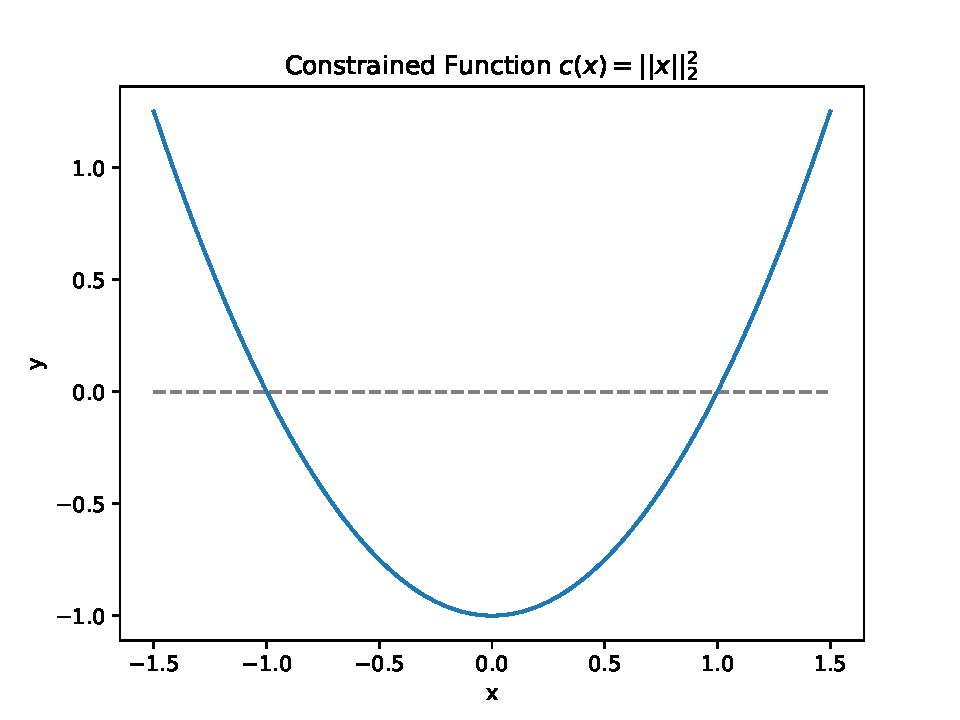
\includegraphics[page=1,width=.7\textwidth]{figs/constrained_22.pdf} 
  \caption{Constrained function $c(x) = \|x\|_{2}^{2} - 1$}
 \end{figure}

\par From the constraint defined above, we can write the constraint function as $c(x) = \|x\|_{2}^{2} - 1$ and illustrate it in Fig~\ref{fig:example23_cons}.  Differentiating $c(x)$ with respect to $x$, we get $\nabla c(x) = x \neq 0$. Therefore, it follows the definition of LFD~\ref{defn:lfd} and the theorem of KKT~\ref{thm:kkt}, which means that every local minimizer of this problem is a KKT point. Now we can write the Lagrangian function:
$$
\mathcal{L}(x, \lambda)=-x^{T} y+\lambda\left(\|x\|_{2}^{2}-1\right)
$$
and the KKT conditions are:
$$
\nabla_x \mathcal{L} = -y+2\lambda x = 0, \quad \|x\|_{2}^{2} = 1
$$
From $-y+2\lambda x = 0$ and $y \neq 0$ defined in the question, we must have $\lambda \neq 0$ and $x = y / 2\lambda$. Combined with $\|x\|_{2}^{2} = 1$, we get 
$$ 
4 \lambda^{2}=\|y\|_{2}^{2} \Leftrightarrow \lambda=\pm \frac{\|y\|_{2}}{2}
$$
\par Therefore, consequently, we have $x = \pm \frac{y}{\|y\|_{2}}$. For each $x$, we can compute its corresponding value of the objective function:
$$
x = \frac{y}{\|y\|_{2}}, -x^{T} y=-\|y\|_{2}
$$
$$
x = -\frac{y}{\|y\|_{2}}, -x^{T} y=\|y\|_{2}
$$ 
\par Obviously, the minimum is achieved $-\|y\|_{2}$ at $x = \frac{y}{\|y\|_{2}}$. 
\par Algorithms for solving constrained problems are various. For basic linear programming, which means that all functions involved are linear, we can transform it into standard form with matrix $A$, then solve the problem using Lagrangian function based on the KKT condition. 
\par Penalty method\citep{YO:05}, a function determining when a point $x$ is feasible or not, is used to replace the constrained problem with an unconstrained one. For a minimization problem $f(x)$, the penalty function $P(x)$ associated with a penalty parameter are introduced to combine with $f(x)$ and now we are going to solve a series of unconstrained problems. These problems have converged solutions of the original constrained problem. 

\subsection{Inequality Constrained Optimization}
\label{sec:ineq-opt}
Similar to equality constrained problems, inequality constrained problem usually defined the solution in a feasible set. In general, the standard form of inequality constrained problem is negative constraints:
$$
\begin{array}{rl}y(x) \in \arg \min _{y \in \mathbb{R}^{m}} & f(x, y) \\ \textrm { subject to } & c_i(x, y) \leq 0, \quad i = 1, \dots, m \end{array}
$$
\par Solutions for inequality constrained problems are various. According to the properties of inequality constraints, active and inactive constraints have different criteria. We aim to find the gradient of the optimal solution, $f\prime (x)$, based on the inequality constrained argmin function. 
 \cite{PE:88} proposed a globally convergent algorithm for solving the minimization of smooth objective function based on smooth inequality constraints. This algorithm is based on the Quasi-Newton~\citep{DJ:77} iteration for the solution of the first order condition of the optimality in KKT. An updated verision of this algorithm, a new QP-free method demonstrated by \cite{QH:00}, emphasizes the feasibility of all iterates. It reformulates the KKT optimality condition Fischer–Burmeister function~\citep{JH:99} for nonlinear complementarity problems. The classical solution is still based on the Lagrange multipliers. \cite{BD:14} proposed that for one-sided inequality constrained problems, it cannot be converted to equality constrained problem. Therefore, it introduced the method minimizing the augumented Lagrangian with respect to $x$ for various value of the Lagrange parameters, which is presented by \cite{PM:69} and \cite{HM:69}: 
 $$
 \begin{aligned} \bar{L}_{c}(x, z, \lambda, \mu)=& f(x)+\lambda^{\prime} h(x)+\frac{1}{2} c|h(x)|^{2} \\ &+\sum_{j=1}^{r}\left\{\mu_{j}\left[g_{j}(x)+z_{j}^{2}\right]+\frac{1}{2} c\left|g_{j}(x)+z_{j}^{2}\right|^{2}\right\} \end{aligned}
 $$
 \par The minimization of this augumented Lagrangian can be found through computing the first order derivative with respect to $z$ explicitly for each fixed $x$. 
\par More recently, \cite{SG:16} introduced a method approximating the gradient of the inequality constrained problem based on ideas from interior-point methods~\citep{BS:04}. It gives a demonstration of log-barrier function, which transforms the original constrained problem into a unconstrained minimization problem.
\begin{equation}
\label{equ:log-barrier}
\phi(x, y)=\sum_{i=1}^{m} \log \left(-c_{i}(x, y)\right)
\end{equation}
\begin{equation}
\label{equ:2.6}
\operatorname{minimize}_{y} \quad t f(x, y)-\sum_{i=1}^{m} \log \left(-c_{i}(x, y)\right)
\end{equation}
Equation~\ref{equ:log-barrier} is the log-barrier function, which takes the sum of the logrithm for all constraints. Then substracting it in the unconstrained minimization problem approximates the original inequality constrained problem. $t$ in Equation~\ref{equ:2.6} is a scaling factor for duality gap control if the solution set is convex. 
\par Similar to the solution for unconstrained and equality constrained problem, minimizing Equation~\ref{equ:2.6} is based on the gradient and hessian of the log-barrier function. Therefore, we can compute the approximation of the inequality constrained objective function. 

\section{Differentiable Neural Network}
\label{sec:differentiable}
If a problem is differentiable, that means the solution of this problem can be back-propagated. In neural networks, back-propagation~\citep{GI:16} is widely used to train the feedforward neural network, especially for supervised learning. Therefore, in deep neural networks, we can treat constrained optimization as an individual layer. Recently, there are several works on end-to-end differentiable convex optimization in the neural network, since this type of layer provides inductive bias for different problems, which is very practical. 
\par OptNet~\citep{AB:17} is a very classical differentiable layer neural network. Each layer in the end-to-end deep neural network is intergraded into optimization problems, which can capture and encode complex dependencies and constraints between hidden variables. It specifically considers the quadratic programs, which are general convex optimization problems. Similarly, SATNet~\citep{WP:19}, a differentiable maximum satisfiability solver, is also intergraded into end-to-end deep learning systems. Besides, it combines the solver with the traditional convolutional network. Both OptNet and SATNet are applied to solving the Sudoku puzzles, which is a very basic constrained logical problem. To make it more general and efficient, \cite{AA:19} demonstrate an approach based on disciplined convex programs, which is a subclass of the classical convex optimization problems. The affine map introduced in this paper represents the disciplined parametrized program. 
\par A fashion application in the differentiable network is the Perspective-n-Points (PnP) solver. \cite{CB:20} present BPnP based on PnP solver, performing geometric optimization in computer vision tasks. It back-propagates gradient through PnP accurately and effectively since there is a differentiable function in the optimizer block. Besides, for blind PnP problems in the 3D computer vision task, \cite{CD:20} propose an end-to-end network based on the differentiating optimization solutions, which is robust and outperforming.  
\par Apart from the above, the differentiable neural network has many practical and powerful applications. \cite{AB:19} introduce a differentiable variant cross-entropy method for non-convex optimization objective function. Again, due to the differentiable feature of the network, the output of the cross-entropy method is differentiable with respect to the parameters in the objective function, even it is non-convex. In 3D reconstruction tasks, some implicit shape and texture are difficult to represent. Hence, \cite{NM:20} introduce a differentiable rendering formulation, which makes the network learn them from input images directly since implicit differentiation can learn the depth gradients. Also, some research has been done to simplify the differentiable neural network since the computational cost and complexity of the differential operators can be very high in different tasks. The architecture proposed by \cite{CR:19} is cheap and efficient, which sets the Jacobian matrix into diagonal and hollow. It also changes the backward progress into automatic differentiation, which is more effective and lightweight. 


\section{Summary}
\label{sec:2summary}
In Chapter~\ref{cha:overviewpart1}, firstly, we introduce the numerical optimization briefly with some necessary conditions and theorems. For the general convex optimization problem, the existence of the local or global optimizers can be determined by the feasible set. Next, the optimality of both unconstrained and constrained problems are discussed. For unconstrained problems, we only need to follow the necessary and sufficient conditions to find the global minimum of the solution. For constrained problems, it should also satisfy the KKT condition. Then we compare existing algorithms on the solution to these problems. Here, for constrained optimization problems, we have to consider the linearity of constraints. Specifically, the activity of inequality constraints can also be solved with different algorithms. Finally, since this thesis is based on the end-to-end differentiable network, some related works of the application are described since these works inspire the deep declarative network in the next chapter. In the next chapter, we are going to describe the deep declarative network in detail with examples. 




